\begin{figure}[htp]
	\centering\capstart{}
	\subfloat[\(\Re\big\{\pixel{S_{1}}\big\},\ \mu=1.00\)] % chktex 21
	{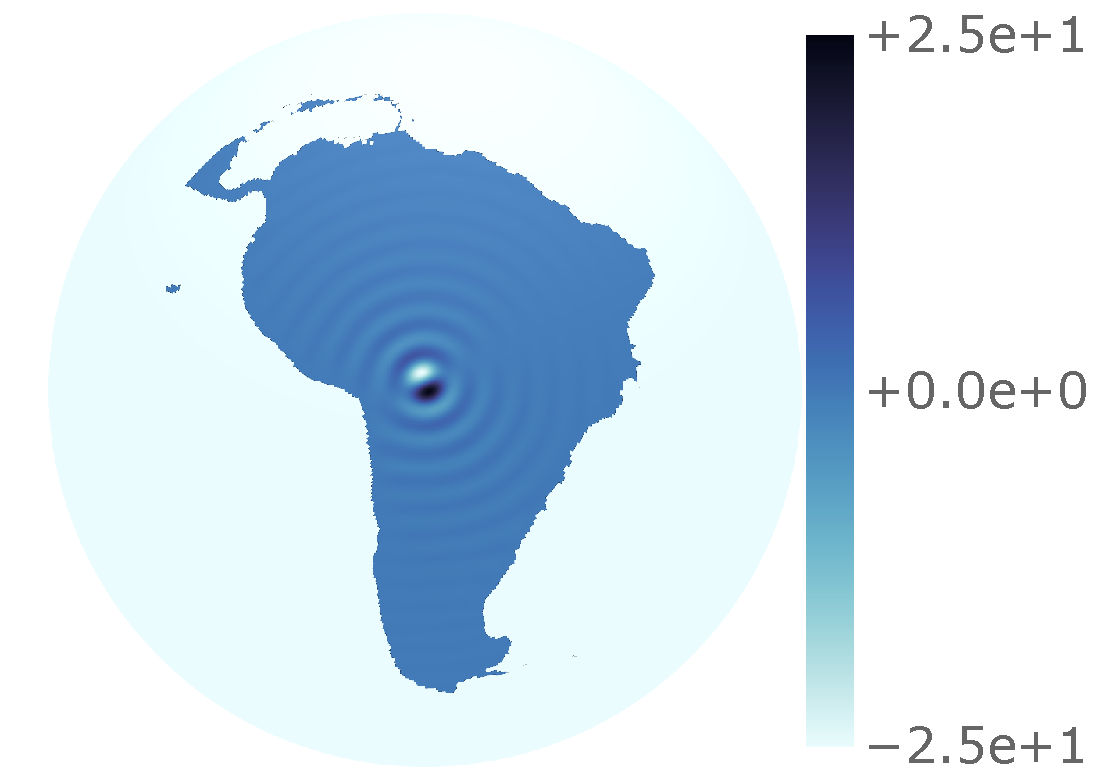
\includegraphics[trim={23 7 3 6},clip,width=.5\textwidth]{slepian_south_america_rank0_lam1-003338e00_L128_res512_real.pdf}} % chktex 8
	\hfill
	\subfloat[\(\Re\big\{\pixel{S_{10}}\big\},\ \mu=1.00\)] % chktex 21
	{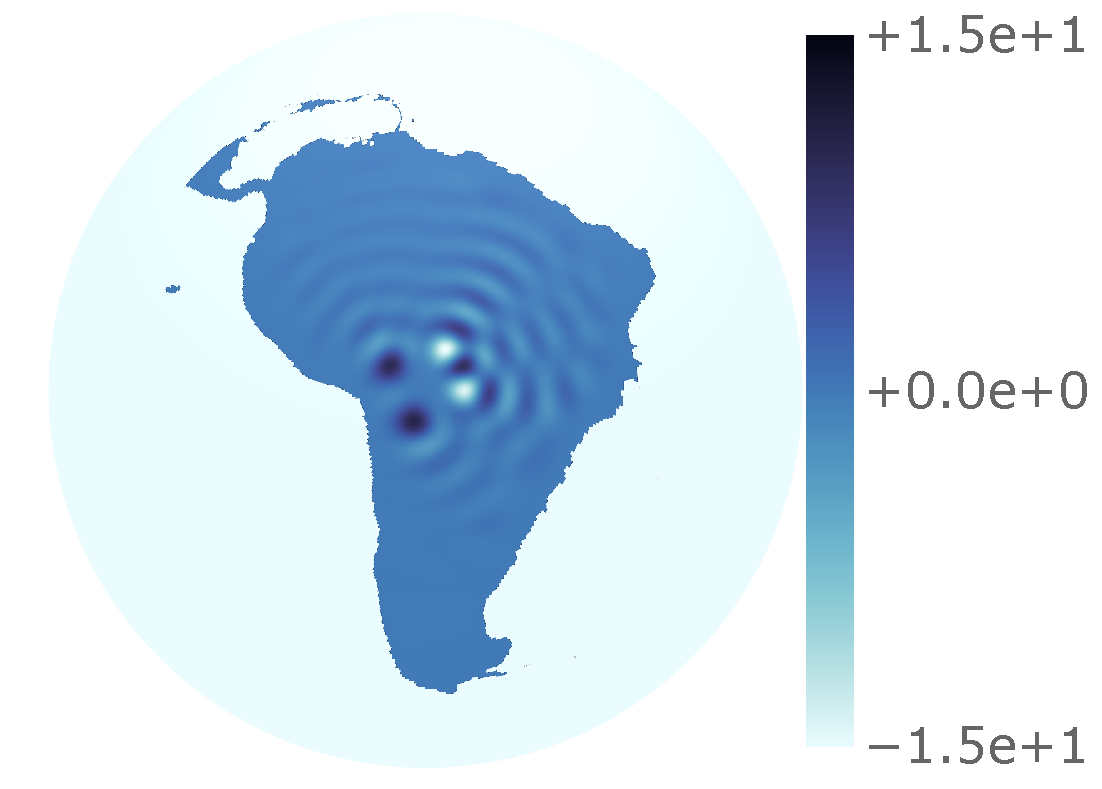
\includegraphics[trim={23 7 3 6},clip,width=.5\textwidth]{slepian_south_america_rank9_lam1-000000e00_L128_res512_real.pdf}} % chktex 8
	\newline
	\subfloat[\(\Re\big\{\pixel{S_{25}}\big\},\ \mu=1.00\)] % chktex 21
	{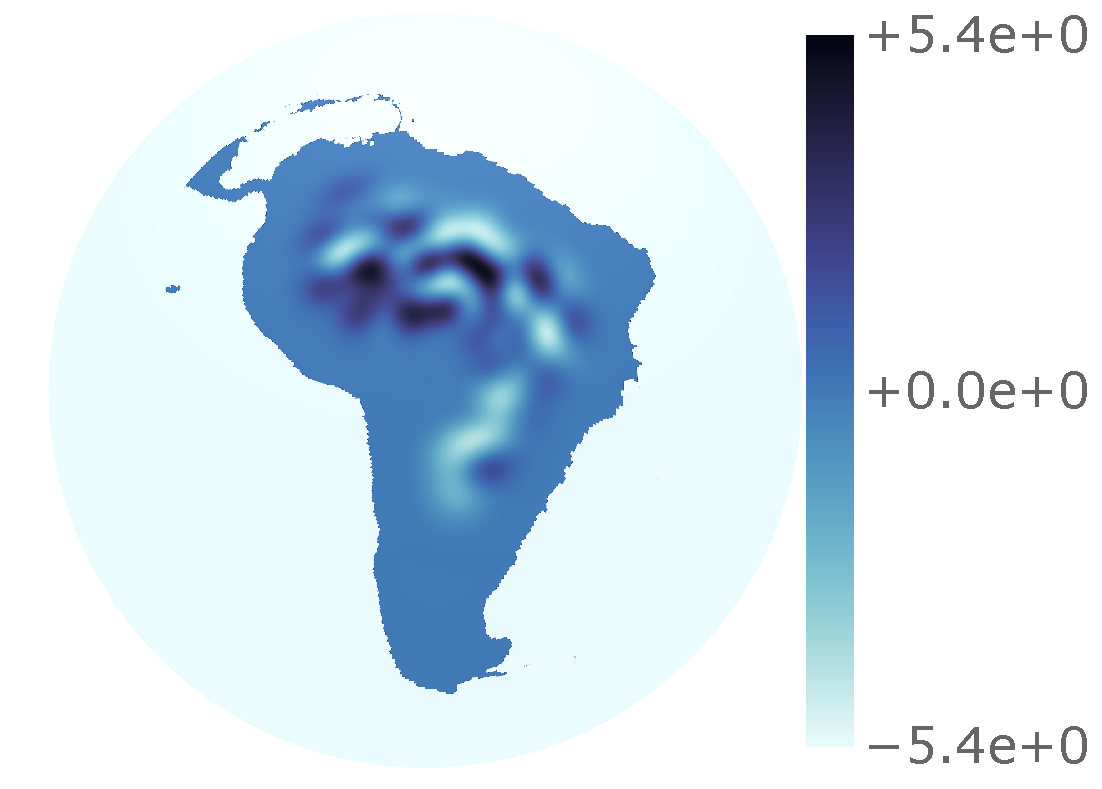
\includegraphics[trim={23 7 3 6},clip,width=.5\textwidth]{slepian_south_america_rank24_lam1-000000e00_L128_res512_real.pdf}} % chktex 8
	\hfill
	\subfloat[\(\Re\big\{\pixel{S_{50}}\big\},\ \mu=1.00\)] % chktex 21
	{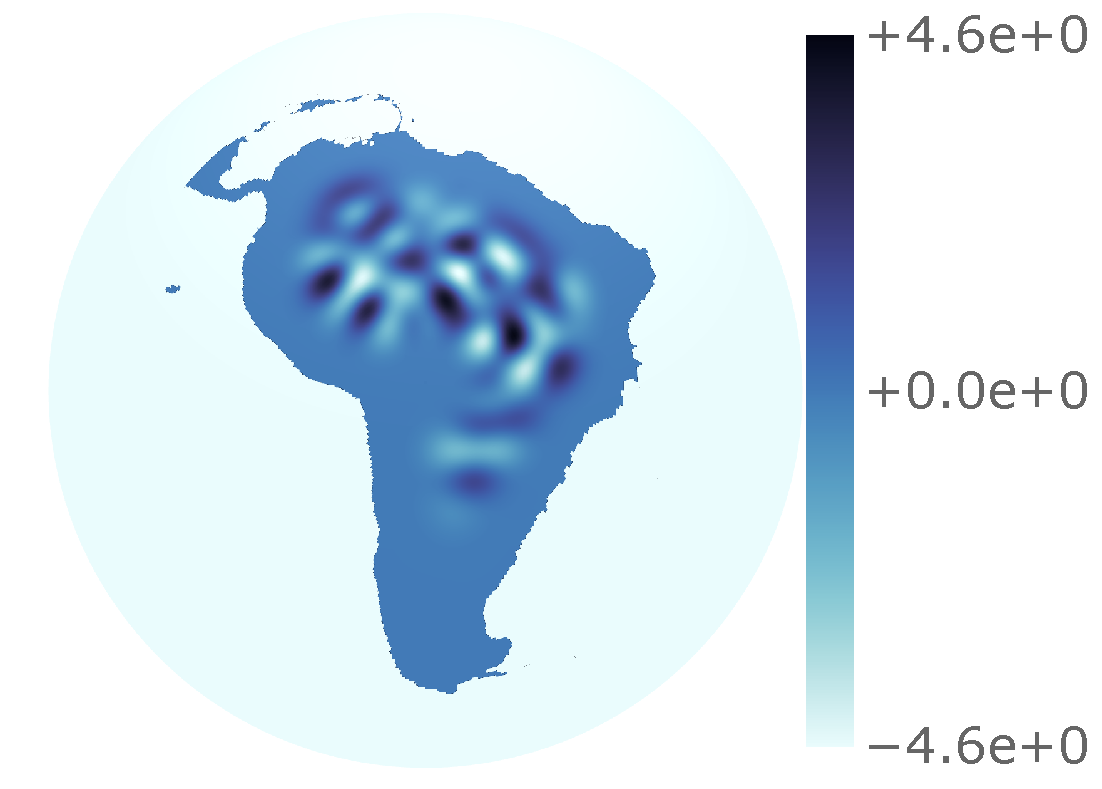
\includegraphics[trim={23 7 3 6},clip,width=.5\textwidth]{slepian_south_america_rank49_lam1-000000e00_L128_res512_real.pdf}} % chktex 8
	\newline
	\subfloat[\(\Re\big\{\pixel{S_{100}}\big\},\ \mu=1.00\)] % chktex 21
	{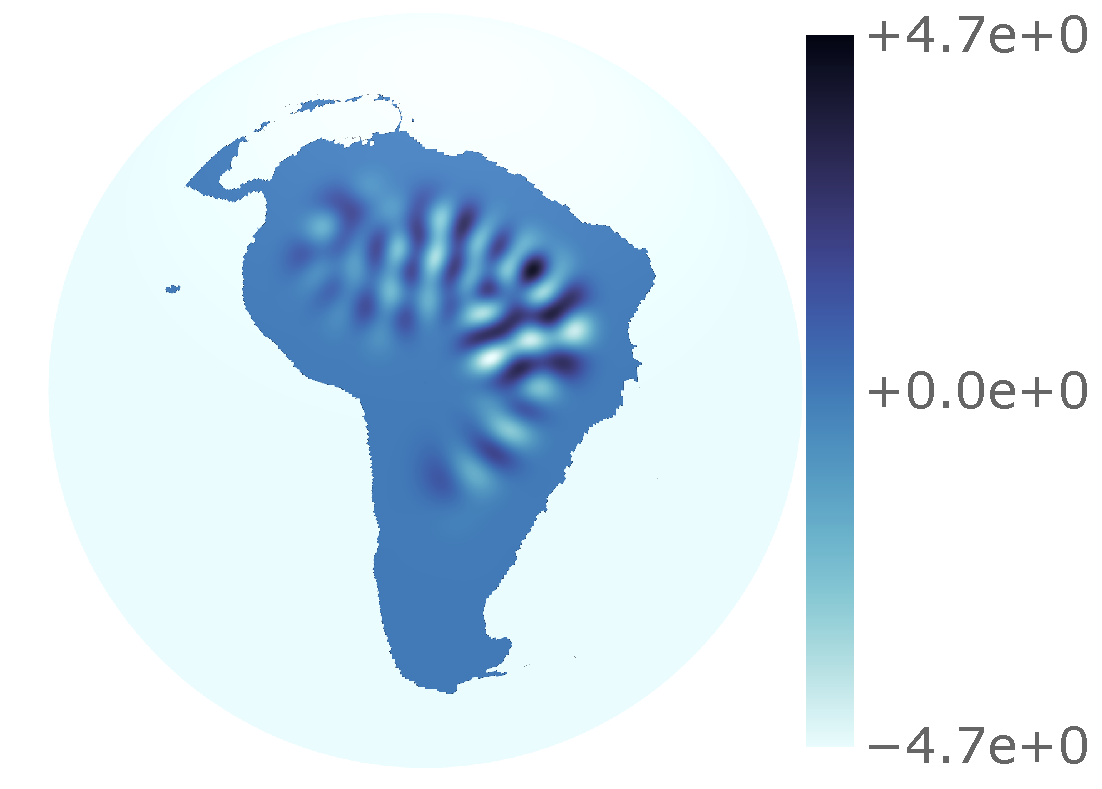
\includegraphics[trim={23 7 3 6},clip,width=.5\textwidth]{slepian_south_america_rank99_lam1-000000e00_L128_res512_real.pdf}} % chktex 8
	\hfill
	\subfloat[\(\Re\big\{\pixel{S_{200}}\big\},\ \mu=1.00\)] % chktex 21
	{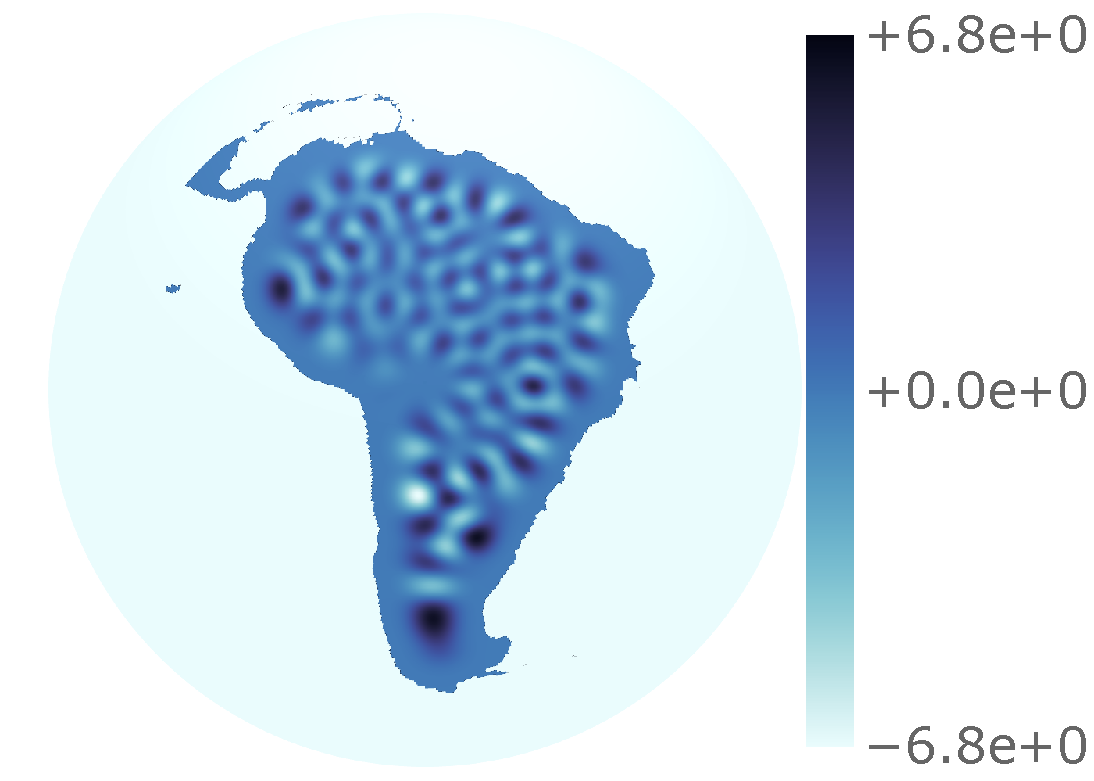
\includegraphics[trim={23 7 3 6},clip,width=.5\textwidth]{slepian_south_america_rank199_lam1-000000e00_L128_res512_real.pdf}} % chktex 8
	\caption[
		Some Slepian functions of the South America region
	]{
		The Slepian functions of the South America region \(S_p(\omega)\) for \(p \in \set{1, 10, 25, 50, 100, 200}\) shown left-to-right, top-to-bottom.
		The corresponding eigenvalue \(\slepian{\mu}\) is a measure of the concentration within the given region \(R\) which remain \(\almost{1}\) for many \(p\) values before decreasing towards zero.
	}\label{fig:chapter3_eigenfunctions}
\end{figure}
